\documentclass[a4paper,10pt,DIV=12]{scrartcl}

\usepackage[ngerman]{babel}
\usepackage[T1]{fontenc}
\usepackage[utf8]{inputenc}

\usepackage{mathptmx}
\usepackage{helvet}
\usepackage{courier}
%
\usepackage{amssymb}
\usepackage{type1cm}        
\usepackage{textcomp}

\usepackage{makeidx}         % allows index generation
\usepackage{graphicx}        % standard LaTeX graphics tool
                             % when including figure files
\usepackage{multicol}        % used for the two-column index
\usepackage[bottom]{footmisc}% places footnotes at page bottom

\usepackage{xcolor}
\usepackage{textcomp}

\usepackage{listings}		% for code highlighting
\lstset{
  basicstyle=\ttfamily,
  showstringspaces=false,
  commentstyle=\color{red},
  keywordstyle=\color{blue},
  breaklines=true,
  language=python,
  basicstyle=\small
}

% listing stuff
\renewcommand{\lstlistingname}{Code-Beispiel}% Listing -> Algorithm
\renewcommand{\lstlistlistingname}{Liste von Code-Beispielen}% List of Listings -> List of Algorithms
\lstset{
captionpos=b
}

\newtheorem{theorem}{Theorem}[section]
\newtheorem{lemma}[theorem]{Lemma}
\newtheorem{proposition}[theorem]{Proposition}
\newtheorem{corollary}[theorem]{Corollary}

\newenvironment{proof}[1][Proof]{\begin{trivlist}
\item[\hskip \labelsep {\bfseries #1}]}{\end{trivlist}}
\newenvironment{definition}[1][Definition]{\begin{trivlist}
\item[\hskip \labelsep {\bfseries #1}]}{\end{trivlist}}
\newenvironment{example}[1][Example]{\begin{trivlist}
\item[\hskip \labelsep {\bfseries #1}]}{\end{trivlist}}
\newenvironment{remark}[1][Remark]{\begin{trivlist}
\item[\hskip \labelsep {\bfseries #1}]}{\end{trivlist}}

\newcommand{\qed}{\nobreak \ifvmode \relax \else
      \ifdim\lastskip<1.5em \hskip-\lastskip
      \hskip1.5em plus0em minus0.5em \fi \nobreak
      \vrule height0.75em width0.5em depth0.25em\fi}


% Registered definieren
\def\SymbReg{\textsuperscript{\textregistered}}


% see the list of further useful packages
% in the Reference Guide
\makeindex             % used for the subject index
                       % please use the style svind.ist with
                       % your makeindex program
%%%%%%%%%%%%%%%%%%%%%%%%%%%%%%%%%%%%%%%%%%%%%%%%%%%%%%%%%%%%%%%%%%%%%

\begin{document}

\author{
% 1st. author
Levin von Hollen\\
% 2nd. author
Tilman Beck\\
}
\title{Implementierung der Cut~\& ~Count-Technik für das
Steinerbaum-Problem}
\maketitle

\setlength{\parindent}{0pt} 
\section{Einleitung}
\label{c:intro} % Always give a unique label
In dieser Arbeit wird die Cut \& Count-Technik aus \cite{cygan_solving_2011} behandelt und eine konkrete Implementierung für das Steinerbaum-Problem dargestellt. 
In Sektion \ref{sec:intro_not} werden wir die Notation einführen, welche für das Verständnis der folgenden Kapitel wichtig ist. 
Die Cut \& Count-Technik benutzt eine angepasste Form einer Nice Tree Decomposition aus \cite{kloks1994}, welche wir in Kapitel \ref{c:ntd} definieren und veranschaulichen.
In Kapitel \ref{c:cc_general} wird die Funktionsweise der Cut \& Count-Technik allgemein erklärt. 
Anschließend wird in Kapitel \ref{c:cc_steiner} die Technik auf das Steinerbaum-Problem angewendet und erläutert. 
Kapitel \ref{c:impl} umfasst unsere Implementierung zum Steinerbaum-Problem, eine kurze Evaluation zu verschiedenen Eingabegrößen, die Diskussion unserer Ergebnisse und einen Ausblick. 
Im letzten Kapitel \ref{c:summary} wird der Inhalt dieser Arbeit zusammengefasst.

\subsection{Notation}
\label{sec:intro_not}
Für den Rest der Arbeit bedienen wir uns der Notation aus der Arbeit \cite{cygan_solving_2011}. 
Die Bezeichnung $G=(V,E)$ beschreibt einen ungerichteten Graphen. Entsprechend beschreiben $V(G)$ und $E(G)$ die Menge der Knoten bzw. Kanten des Graphen $G$. 
Die Bezeichung $G[X]$ einer Knotenmenge $X \subseteq V(G)$ steht für den Subgraphen, der von $X$ erzeugt wird. Für eine Menge an Kanten $X \subseteq E$ beschreibt $V(X)$ die Menge der Endknoten der Kanten aus $X$ und $G[X]$ den Subgraphen $(V,X)$. 
Die Knotenmenge für eine Menge von Kanten $X$ im Graphen $G[X]$ ist diesselbe wie im Graphen $G$.

Mit einem \glqq Schnitt\grqq ~einer Menge $X \subseteq V$ ist das Paar $(X_1,X_2)$ mit den Eigenschaften $X_1 \cap X_2 = \emptyset,X_1 \cup X_2 = X$ gemeint. 
$X_1$ und $X_2$ werden als linke und rechte \glqq Seiten\grqq des Schnittes bezeichnet. 

Eine Zusammenhangskomponente beschreibt eine Teilmenge eines Graphen, die zusammenhängend ist.

Die Zahl $cc(G)$ eines Graphen $G$ beschreibt die Anzahl der Zusammenhangskomponenten (\glqq \textbf{c}onnected \textbf{c}omponents\grqq).

Für zwei Bags $x,y$ eines Baums mit Wurzelknoten gilt, dass $y$ ein Nachkomme von $x$ ist, falls es möglich ist ausgehend von $y$ einen Weg zu $x$ zu finden, der im Baum nur in Richtung des Wurzelknotens verläuft. 
Insbesondere ist $x$ sein eigener Nachkomme.

Für zwei Integer $a,b$ sagt die Gleichung $a \equiv b$ aus, dass $a$ genau dann gerade ist, wenn auch $b$ gerade ist.
Zudem wird Iverson's Klammernotation verwendet. 
Falls $p$ ein Prädikat ist, dann sei $[p]$ 1 (0) falls $p$ wahr (unwahr) ist.
Falls $\omega:U\rightarrow {1,\dots,N}$, so bezeichnet $\omega(S)=\sum_{e\in S} \omega(e)$ für $S \subseteq U$.

Für eine Funktion $s$ mit $s[v \rightarrow \alpha]$ schreiben wir die Funktion $s \ {(v,s(v))}\cup{(v,\alpha)}$. Diese Definition funktioniert unabhängig davon, ob $s(v)$ bereits definiert wurde oder nicht.

%%%%%%%%%%%%%%%%%%%%% chapter.tex %%%%%%%%%%%%%%%%%%%%%%%%%%%%%%%%%
%
% sample chapter
%
% Use this file as a template for your own input.
%
%%%%%%%%%%%%%%%%%%%%%%%% Springer-Verlag %%%%%%%%%%%%%%%%%%%%%%%%%%
%\motto{Use the template \emph{chapter.tex} to style the various elements of your chapter content.}
\chapter{(Nice) Tree Decomposition}
\label{c:ntd} % Always give a unique label
% use \chaptermark{}

\section{Tree Decomposition}
\label{sec:ntd_td}
\begin{definition}
(Tree decomposition, \cite{robertson1984graph}). Eine Tree Decomposition \textit{eines (ungerichteten oder gerichteten) Graphen $G$ ist ein Baum $\mathbb{T}$ in dem jedem Knoten $x \in \mathbb{T}$ eine Menge von Knoten $B_x \subseteq V$ (genannt \glqq Bag\grqq) zugeordnet ist, so dass 
\begin{itemize}
\item für jede Kante $uv \in E$ existiert ein $x \in \mathbb{T} $, so dass $u,v \in B_x$
\item falls $v \in B_x$ und $v \in B_y$, dann $v \in B_z$ für alle $z$ auf dem Pfad von $x$ nach $y$ in $\mathbb{T}$
\end{itemize}
}
\end{definition}

Das Konzept der Tree Decomposition wurde 1976 von Rudolf Halin \cite{Halin1976} eingeführt. Sie dient dazu die Baumweite zu definieren und Berechnungsprobleme auf Graphen schneller zu lösen.

Die Baumweite ist eine Zahl und beschreibt die \glqq Baum-Ähnlichkeit\grqq ~eines Graphen. Die Baumweite $tw(\mathbb{T})$ einer Tree Decomposition $\mathbb{T}$ ist die Größe des größten Bags minus eins. Die Baumweite eines Graphen $G$ ist die minimale Baumweite aller möglichen Tree Decompositions von $G$.

Ein Beispiel für eine Tree Decomposition ist in Abbildung \ref{fig:td_2} gegeben. Der Ursprungsgraph ist in Abbildung \ref{fig:td_1}.

\begin{figure}
\centering
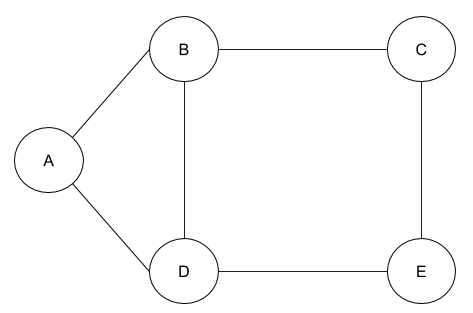
\includegraphics[width=0.5\textwidth]{./imgs/TD_1.png}
\caption{Ursprungsgraph für eine Tree Decomposition}
\label{fig:td_1}
\end{figure}

\begin{figure}
\centering
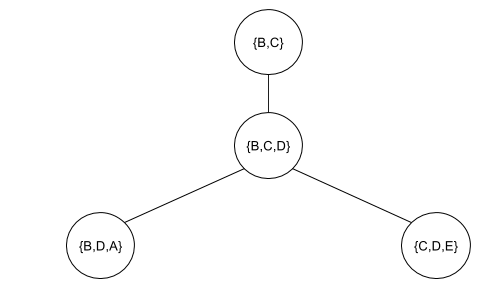
\includegraphics[width=0.6\textwidth]{./imgs/TD_2.png}
\caption{Eine Tree Decomposition für den in Abbildung \ref{fig:td_1} gegebenen Ursprungsgraphen}
\label{fig:td_2}
\end{figure}

\section{Nice Tree Decomposition}
\label{sec:ntd_ntd}
Kloks \cite{kloks1994} führte die sogenannte Nice Tree Decomposition ein, welche oft für Algorithmen mit dynamischen Programmen genutzt werden. Da in Sektion \ref{sec:ntd_req} weitere Modifikationen auf Basis der Nice Tree Decomposition eingeführt werden, wird die hier vorgestellte Nice Tree Decomposition als \textit{standardmäßige Nice Tree Decomposition} bezeichnet.

\begin{definition}
Eine standardmäßige Nice Tree Decomposition ist eine \textit{Tree Decomposition, für die gilt:
\begin{itemize}
\item jeder Bag besitzt höchstens zwei Kind-Knoten
\item falls ein Bag $x$ zwei Kind-Knoten $l,r$ besitzt, dann gilt $B_x=B_l=B_r$
\item falls ein Bag $x$ einen Kind-Knoten besitzt, dann gilt entweder $|B_x|=|B_y| + 1$ und $B_y \subseteq B_x$ oder $|B_x| + 1 = |B_y|$ und $B_x \subseteq B_y$
\end{itemize}
}
\end{definition}

\section{Weitere Modifikationen}
\label{sec:ntd_req}
Für den von \cite{cygan_solving_2011} beschriebenen Algorithmus wird die standardmäßige Nice Tree Decomposition zusätzlich noch auf folgende Weise modifiziert:
\begin{definition}
(Nice Tree Decomposition). Eine Nice Tree Decomposition \textit{ist eine Tree Decomposition mit einem speziellen Bag $z$ (Wurzel) mit $B_z=\emptyset$ und in der jeder Bag einer der folgenden Arten entspricht:
\begin{itemize}
\item \textbf{Leaf Bag}: ein Blatt $x$ aus $\mathbb{T}$ mit $B_x=\emptyset$ .
\item \textbf{Introduce Vertex Bag}: ein innerhalb von $\mathbb{T}$ liegender Knoten $x$ mit einem Kind-Knoten $y$ für den gilt $B_x=B_y \cup \{v\}$ für ein $v \notin B_y$. Dieser Bag führt den Knoten $v$ ein.
\item \textbf{Introduce Edge Bag}: ein innerhalb von $\mathbb{T}$ liegender Knoten $x$, der mit der Kante $uv \in E$ gekennzeichnet ist und einen Kind-Knoten $y$ mit $u,v \in B_x = B_y$ besitzt. Dieser Knoten führt die Kante $uv$ ein.
\item \textbf{Forget Bag}: ein innerhalb von $\mathbb{T}$ liegender Knoten $x$ mit einem Kind-Knoten $y$, für den gilt $B_x=B_y\backslash \{v\}$ für ein $v \in B_y$. Dieser Bag vergisst den Knoten $v$.
\item \textbf{Join Bag}: ein innerhalb von $\mathbb{T}$ liegender Knoten $x$ mit zwei Kind-Knoten $l,r$, für die $B_x=B_r=B_l$ gilt. 
\end{itemize}
Zusätzlich wird gefordert, dass jede Kante aus $E$ genau einmal eingeführt wird.
}\\

Ein Beispiel für eine Nice Tree Decomposition ist in Abbildung \ref{fig:td_3}.
\begin{figure}
\label{fig:td_3}

  \centering
    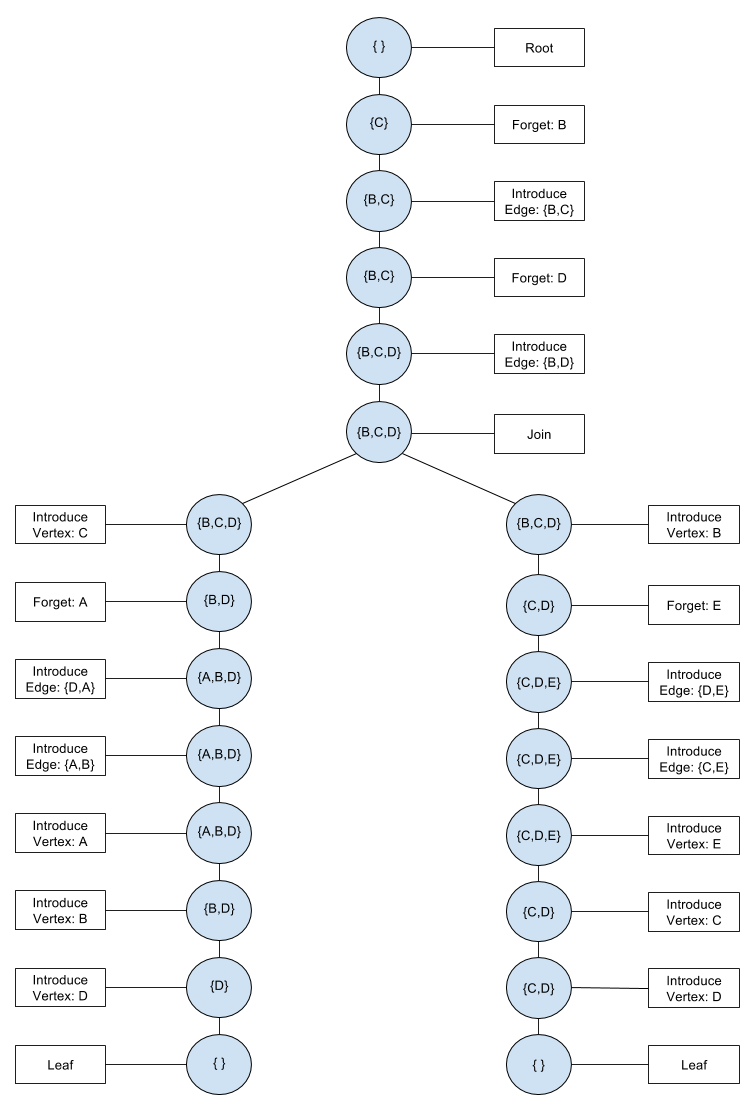
\includegraphics[width=1.0\textwidth]{./imgs/TD_3.png}
  	\caption{Eine Nice Tree Decomposition für den Ursprungsgraphen in Abbildung \ref{fig:td_1}}
\end{figure}

Sei eine Tree Decomposition gegeben, kann eine standardmäßige Nice Tree Decomposition von gleicher Breite in polynomieller Zeit gefunden werden \cite{kloks1994}. Der Algorithmus für eine standardmäßige Nice Tree Decomposition kann in der selben Laufzeit  modifizert werden, so dass das Ergebnis zusätzlich die o.g. Kriterien erfüllt.
\end{definition}


\chapter{Cut \& Count-Technik}
\label{c:cc_general}

\section{Einführendes}
\label{sec:cc_intro}
Die Cut \& Count-Technik aus \cite{cygan_solving_2011} wird benutzt um Zusammenhangs-Probleme von Graphen zu lösen.
Dabei handelt es sich um Graphen-Probleme, bei denen zusammenhängende Submengen der Knoten gefunden werden müssen, die problemspezifische  Eigenschaften erfüllen müssen. 
Die Technik setzt sich aus den beiden Teilen \glqq Cut\grqq ~, \glqq Count\grqq ~zusammen (siehe Sektion \ref{sec:cc_cc}) und kann auf mehrere Probleme angewendet werden, u.A. Längster Weg, Steinerbaum oder Feedback Vertex Set.

Das Ergebnis ist ein Monte-Carlo-Algorithmus, welcher eine Aussage über die Existenz einer (oder mehrerer) Lösungen gibt. Dies ist in Sektion \ref{sec:cc_monte} erläutert.
Mithilfe von Randomisierung beschränkt die Technik die Anzahl der Lösungsmengen mit einer Wahrscheinlichkeit, die durch das Isolation-Lemma begrenzt werden kann. Dies wird in Sektion \ref{sec:cc_iso} näher erklärt.


\section{Cut \& Count}
\label{sec:cc_cc}
Sei $\mathcal{S}$ die Menge der Lösungen für das Graphenproblem. 
Dann entscheidet Cut \& Count ob diese Menge leer ist. 
Dazu kann Cut \& Count folgendermaßen aufgeteilt werden:

\subsection{Cut}
\label{ssec:cc_cut}
Die Zusammenhangs-Bedingung aus dem Graphenproblem wird abgeschwächt, indem eine Menge von Lösungskandidaten $\mathcal{R} \supseteq \mathcal{S}$ betrachtet wird. 
Zusätzlich wird die Menge $\mathcal{C}$ von Paaren $(X,C)$ betrachtet, wobei $X \in \mathcal{R}$ und $C$ einen konsistenten Schnitt beschreibt. 

\subsection{Count}
\label{ssec:cc_count}
Berechne $|\mathcal{C}|$ modulo 2 mithilfe der Prozedur $\mathtt{countC}$ (siehe Sektion \ref{ssec:impl_countc}). 
Dadurch werden alle unzusammenhängenden Lösungskandidaten $X \in \mathcal{R} \setminus \mathcal{S}$ ignoriert, da die Anzahl derer mit einer geraden Anzahl von konsistenten Schnitten konsistent sind. Es bleiben die zusammenhängenden Lösungskandidaten $x \in \mathcal{S}$ übrig. 

Der Algorithmus \glqq zählt\grqq ~nicht die Lösungen, sondern die Anzahl der Lösungskandidaten, die einen konsistenten Schnitt bilden.

\section{Monte-Carlo-Algorithmus}
\label{sec:cc_monte}
Ein Monte-Carlo-Algorithmus ist ein randomisierter Algorithmus, welcher mit einer nach oben beschränkten Wahrscheinlichkeit ein falsches Ergebnis liefern darf. 
Für die Cut \& Count-Technik bedeutet dies, dass der hervorgegangene Algorithmus niemals ein falsch-positives Ergebnis\footnote{Der Algorithmus gibt eine positive Antwort auf das Problem, obwohl keine Lösung existiert} ausgeben kann, aber zu einer gewissen Wahrscheinlichkeit ein falsch-negatives Ergebnis\footnote{Der Algorithmus gibt eine negative Antwort auf das Problem, obwohl eine Lösung existiert.}. 
Die Wahrscheinlichkeit eines falsch-negativ wird durch das Isolations-Lemma begrenzt. 
Die Ausgabe eines falsch-negativ unterliegt einer bestimmten Wahrscheinlichkeit. Daher ist sinnvoll den Algorithmus in diesem Fall mehrmals hintereinander ausführen. Es begünstigt die Wahrscheinlichkeit eine Lösungsmenge zu finden, falls diese existiert.

Der Monte-Carlo-Algorithmus erreicht folgende Laufzeiten für einige bekannte Zusammenhangs-Probleme bei Graphen, wobei $t$ die Braumbreite der Tree Decomposition beschreibt:
\begin{itemize}
\item Steinerbaum in $3^t |V|^{O(1)}$
\item Feedback Vertex Set in $3^t|V|^{O(1)}$
\item ...
\end{itemize}

\section{Isolation Lemma}
\label{sec:cc_iso}
Da im Count-Teil die Menge $|\mathcal{C}|$ modulo 2 berechnet wird, muss sichergestellt werden, dass die Menge der Lösungen begrenzt wird. 
Für eine gerade Anzahl von Lösungen würde der Algorithmus sonst ein falsch-negatives Ergebnis liefern, da jede gerade Anzahl durch die Modulo-Operation nicht erkannt wird. 
Daher muss die Lösungsmenge reduziert werden. Dafür wird auf das Isolations-Lemma zurückgegriffen. Dieses ist wie folgt definiert:

\begin{definition}
Isolation Lemma\\
 A function $\omega : U \rightarrow \mathbb{Z}$ isolates a set family $\mathcal{F} \subseteq 2^U$ if there is a unique $S' \in \mathcal{F}$ with $\omega (S')=min_{S \in \mathcal{S}} \omega(S)$\\
\end{definition}

In der Arbeit \cite{cygan_solving_2011} wird das Isolations-Lemma in Lemma 2.5 verwendet, um folgende Aussage über die Wahrscheinlichkeit der Isolation auszusagen:\\
\\Let $\mathcal{F} \subseteq 2^U$ be a set family over a universe $U$ with $|\mathcal{F}| > 0$. For each $u \in U$ ,
choose a weight $\omega(u) \in {1, 2, . . . , N }$ uniformly and independently at random. Then
\begin{center}
$prob[\omega$ isolates $\mathcal{F}]\geq 1 - \frac{|U|}{N}$
\end{center}

Durch die Wahl eines großen $N$ kann die Wahrscheinlichkeit eines falsch-negativ reduziert werden. Dies geht mit einer Erhöhung der Laufzeit des Algorithmus einher.

%%%%%%%%%%%%%%%%%%%%% chapter.tex %%%%%%%%%%%%%%%%%%%%%%%%%%%%%%%%%
%
% sample chapter
%
% Use this file as a template for your own input.
%
%%%%%%%%%%%%%%%%%%%%%%%% Springer-Verlag %%%%%%%%%%%%%%%%%%%%%%%%%%
%\motto{Use the template \emph{chapter.tex} to style the various elements of your chapter content.}
\chapter{Cut \& Count für das Steinerbaum-Problem}
\label{c:cc_steiner}

\section{Steinerbaum}
\label{sec:steiner}
\begin{definition}
Steinerbaum-Problem\\
\textbf{Eingabe}: Sei $G = (V, E)$ ein ungerichteter Graph, $T \subseteq V$ eine Menge von Terminalknoten und $k$ eine positive Ganzzahl. \\
\textbf{Problemstellung}: Gibt es eine Menge $X \subseteq V$ der Kardinalität $k$, so dass $T \subseteq X$ und $G[X]$ zusammenhängend ist?
\end{definition}

Bei dem Steinerbaum-Problem handelt es sich um ein connectivity-Typ Problem. In einen gegebenen Graphen sind einige Knoten als Terminale makiert. Nun wird nach einem Subgraphen innerhalb des Ursprungsgraphen gesucht, der alle Terminale enthält und aus k vielen Knoten insgesamt besteht. Desweiteren müssen alle Knoten innerhalb des Subgraphen über Kanten untereinander erreichbar sein.

\section{Cut}
\label{sec:st_cut}
Zu beginn des Cut-Teils wird eine zufällige Gewichtsfunktion $\omega:V\rightarrow \{1,\dots,N\}$ definiert. Diese wird für die Isolation der Lösungsmenge verwendet.\\
Desweiteren wird im Cut-Teil die Menge $\mathcal{R}_W$ definiert. Sie ist die Menge aller Teilmengen von $X$ aus $V$ mit $T \subseteq X$, $\omega(X)=W$ und $|X|=k$. Somit stellt die Menge $\mathcal{R}_W$ die Menge aller Lösungskandidaten dar.\\
Eine weitere zu definierende Menge ist $\mathcal{S}_W=\{X \in \mathcal{R}_W | G[X]$ ist zusammenhängend$\}$. Somit bildet die Menge $\mathcal{S}_W$ Lösungen für ein gegebenes bestimmtes Gewicht $W$.\\
$\cup_W \mathcal{S}_W$ bildet so die Lösungsmenge. Gibt es nun ein Gewicht $W$ für das die Menge nicht leer ist, so gibt der Algorithmus eine positive Antwort.\\
Von der Menge der Terminalknoten wird ein Terminal als $v_1$-Terminal festgelegt. Dieses dient dazu, dass bei der Bildung von konsistenten Schnitten kein Schnitt doppelt gezählt wird.\\
Die konsistenten Schnitte werden in der Menge  $\mathcal{C}_W$ beschrieben. Diese bilden die Menge aller Subgraphen, die einen konsistenten Schnitt $(X,(X_1,X_2))$ bilden, wobei $X\in \mathcal{R}_W$ und $v_1 \in X_1$.
\begin{figure}
\label{fig:st_cut}
  \centering
    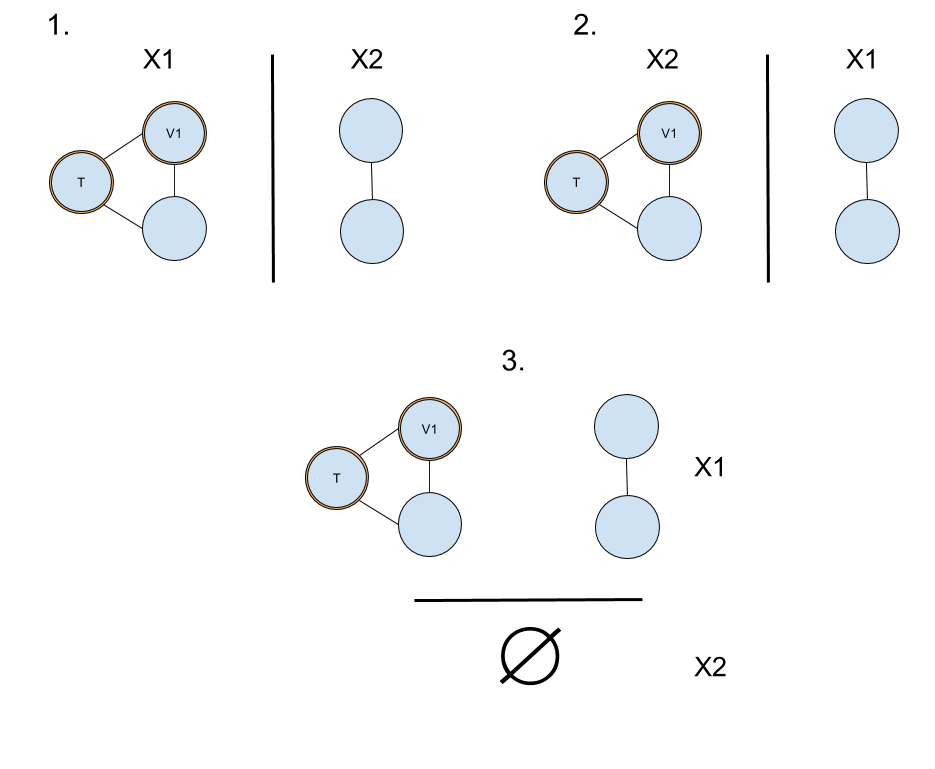
\includegraphics[width=1.0\textwidth]{./imgs/terminal_v1.png}
  	\caption{Konsistente Schnitte ohne Beschränkung $v_1 \in X_1$. Man sieht, dass die konsistenten Schnitte 1 und 2 identisch sind.}
\end{figure}

Die Anzahl der konsistenten Schnitte sind in Lemma 3.3 in \cite{cygan_solving_2011} definiert:\\
Let $G=(V,E)$ be a graph and let $X$ be a subset of vertices such that $v_1 \in X \subseteq V$. The number of consistently cut subgraphs $(X,(X_1,X_2))$ such that $v_1 \in X_1$ is equal to $2^{cc(G[X])-1}$.

Beweis: Per Definition ist bekannt, dass für jeden konsistenten Schnitt $(X,(X_1,X_2))$ und Connected Component $C$ aus $G[X]$ $C$ entweder in $X_1$ oder in $X_2$ enthalten sein muss. Für die Connected Component, die $v_1$ enthält ist die Wahl der Submenge fix. Für alle anderen Connected Components kann die Zugehörigkeit von Submengen frei gewählt werden. Daher erhalten wir $2^{cc(G[X])-1}$ verschiedene konsistente Schnitte.

\section{Count}
\label{sec:st_count}
Aus Lemma 3.3 ist bekannt: $|\mathcal{C}|=\sum_{X \in \mathcal{R}} 2^{cc(G[X])-1}$. Wir legen $W$ fest und ignorieren die Indices: $|\mathcal{C}| \equiv |\{X \in \mathcal{R} |cc(G[X]) = 1\}| = |\mathcal{S}|$. Das bedeutet, dass die Anzahl der konsistenten Schnitte eines Graphen modulo zwei gleich der Anzahl der Lösungen ist. Im Lemma 3.4 trifft das Paper dazu eine Aussage: Let $G,$ $\omega$, $\mathcal{C}_W$ and $\mathcal{S}_W$ be as defined above. Then for every $W$, $|\mathcal{S}_W| \equiv |\mathcal{C}_W|$.

\section{Dynamisches Programm}
\label{sec:dynP}

$|\mathcal{C}_W|$ modulo $2$ kann mit dynamischen Programm auf der NTD $\mathbb{T}$ berechnet werden.
für jeden Bag $x \in \mathbb{T}$, integers $0 \leq i \leq k,0 \leq w \leq kN$ und Färbung $s \in \{0,1_1,1_2 \}^{B_x}$ definiere:
\begin{itemize}
\item $\mathcal{R}_x(i,w)=\{X \subseteq V_x | (T \cap V_x) \subseteq X$ $\wedge$ $|X| = i$ $\wedge$ $\omega (X) = w \}$
\item $\mathcal{C}_x (i,w) =\{ (X,(X_1,X_2)) | X \in \mathcal{R}_x(i,w)$ $\wedge$ $(X,(X_1,X_2))$ is a consistently cut subgraph of $G_x$ $\wedge$ $(v_1 \in V_x \Rightarrow v_1 \in X_1 \} $
\item $\mathcal{A}_x(i,w,s)=| \{ (X,(X_1,X_2)) \in \mathcal{C}_x(i,w) | (s(v) = 1_j \Rightarrow v \in X_j)$ $\wedge$ $(s(v)=0 \Rightarrow v \notin X \} |$
\end{itemize}
Die Färbungen der Knoten gibt an, ob sie zu einem konsistenten Schnitt gehören und wenn ja zu welcher der beiden Teilmengen des konsistenten Schnitts sie gehören.
Färbung $s \in \{0,1_1,1_2 \}^{B_x}$  der Knoten aus $B_x$ bzgl. der Menge $C_x$
\begin{itemize}
\item $s[v] = 0 \Rightarrow v \notin X$
\item $s[v] = 1_1 \Rightarrow v \in X_1$ 
\item $s[v] = 1_2 \Rightarrow v \in X_2$ 
\end{itemize}
$A_x(i,w,s)$ zählt alle Möglichkeiten die Knoten gemäß der Definition zu färben.
Ob der Algorithmus eine Lösung gefunden hat, kann aus der $k \times kN$-Datenmatrix des Wurzel-Knotens ausgelesen werden. Dieser Zugriff ist konstant in $\mathcal{O}(1)$\\
Im dynamischen Programm werden die folgenden Berechnungsregeln für jede $A_x(i,w,s)$ Matrix eines Bags angewandt. Zur Vereinfachung der Notation beschreibt im folgenden $v$ den neu eingeführten Vertex. $y$ und $z$ stehen für das linke bzw. das rechte Kind:
\begin{itemize}
\item \textbf{Leaf bag}:
\begin{itemize}
\item $A_x=(0,0,\emptyset) = 1$\\Leaf bags enhalten keine Knoten, daher werden sie mit einem Initialwert gefüllt.
\end{itemize}
\item \textbf{Introduce vertex v}:
\begin{itemize}
\item $A_x=(i,w,s[v\rightarrow 0]) = [v \notin T]A_y(i,w,s)$\\ Ist der eingeführte Vertex kein Terminal, so wird der Wert aus dem Bag des Kindes übernommen.
\item $A_x=(i,w,s[v\rightarrow 1_1]) = A_y(i-1,w-w(v),s)$\\ Reduziere beim Zugriff auf den Bag des Kindes i um 1 und ziehen das Gewicht des eingeführten Knoten ab. Übernehme den Wert.
\item $A_x=(i,w,s[v\rightarrow 1_2]) =[v \neq v_1] A_y(i-1,w-w(v),s)$\\ Ist der eingeführte Vertex nicht das speziell gewählte Terminal so verfahre wie bei $1_1$.
\end{itemize}
\item \textbf{Introduce edge uv}
\begin{itemize}
\item $A_x(i,w,s) = [s(u) = 0 \vee s(v) = 0 \vee s(u) = s(v)]A_y(i,w,s)$\\ Ist einer der Verticies $0$ gefärbt oder sind beide gleich gefärbt, so wird der Wert aus dem Bag des Kindes übernommen.
\end{itemize}
\item \textbf{Forget vertex v}
\begin{itemize}
\item $A_x(i,w,s) = \sum\limits_{\alpha \in {0,1_1,1_2}} A_x(i,w,s[v \rightarrow \alpha]) $\\ Es wird die Summe gebildet über alle Färbungen des vergessenen Vertex im Bag des Kindes.
\end{itemize}
\item \textbf{Join bag}
\begin{itemize}
\item $A_x(i,w,s) = \sum\limits_{i_1+i_2=i+|s^{-1}({1_1,1_2})|} \sum\limits_{w_1+w_2=w+w(s^{-1}({1_1,1_2}))} A_y(i_1,w_1,s)A_z(i_2,w_2,s) $\\In der inneren Summe wird über die Gewichte innerhalb beider Bags der Kinder iteriert. Ist deren Summe gleich der Summe von $w$ und der Summe der Gewichte von Knoten mit der Färbung $1_1$ und $1_2$, so werden sie akkumuliert.
\\In der äußeren Summe wird über den Parameter $i$ der Bags der Kinder iteriert. Ist die Summe gleich der Summe von $i$ und der Anzahl der Knoten die $1_1$ und $1_2$ gefärbt sind, so werden sie akkumuliert.
\end{itemize}
\end{itemize}
Da alle Berechnungen der Bags jeweils nur von den Werten des Kindes abhängig sind, kann das Ergebnis des Algorithmus im Wurzelknoten ausgelesen werden. Die Matrix des Wurzelknotens $A_r(k,W,\emptyset)$ enthält an den Stellen k und W eine 1, zu denen es eine Lösung der Größe k mit Gesamtgewicht W existiert. Kleinere Kardinalitäten können hierbei auch direkt überprüft werden.

\section{Monte-Carlo Algorithmus und Laufzeit}
\label{sec:mc_alg}
Im Theorem 3.6 des Papers wird zusammenfassend erwähnt:
\begin{theorem}
There exists a Monte-Carlo algorithm that given a tree decomposition of width $t$ solves STEINER TREE in $3^t|V|^{\mathcal{O}(1)}$ time. The algorithm cannot give false positives and may give false negatives with probability at most 1/2.
\end{theorem}

Die Laufzeit setzt sich wie folgt zusammen:
\begin{itemize}
\item $3^t$:\\ Da alle Knoten drei verschiedene Färbungen annehmen können und über all diese iteriert werden muss, erhalten wir $3^t$ verschiedene Färbungen. Hierbei ist die \textit{treewidth} der Falschenhals. Das Dynamische Programm berechnet nur die Färbungen für alle im Bag enthaltenen Verticies.
\item $|V|^{\mathcal{O}(1)}$:\\ Kommt durch die beiden Input-Parameter k und N.
\item Die Wahrscheinlichkeit von 1/2 für falsch-negativ entsteht durch die Gewichtsfunktion $\omega:V\rightarrow \{1,\dots,N\}$ und durch das Isolations-Lemma. 
\end{itemize}
%%%%%%%%%%%%%%%%%%%%% chapter.tex %%%%%%%%%%%%%%%%%%%%%%%%%%%%%%%%%
%
% sample chapter
%
% Use this file as a template for your own input.
%
%%%%%%%%%%%%%%%%%%%%%%%% Springer-Verlag %%%%%%%%%%%%%%%%%%%%%%%%%%
%\motto{Use the template \emph{chapter.tex} to style the various elements of your chapter content.}
\chapter{Implementierung}
\label{c:impl} % Always give a unique label
% use \chaptermark{}
% to alter or adjust the chapter heading in the running head

\section{Nice Tree Decomposition}
\label{sec:impl_ntd}
Es wurde ein Algorithmus entwickelt, der als Eingabe eine standardmäßige Nice Tree Decomposition $\mathbb{T}$ eines Graphen $G$ erhält und eine Nice Tree Decomposition (siehe Kapitel \ref{sec:impl_ntd}) ausgibt. Da der Fokus dieser Arbeit auf der Implementierung des dynamischen Programms des Cut \& Count-Algorithmus liegt, wurde der Algorithmus nicht hinsichtlich der in \cite{kloks1994} beschriebenen polynomiellen Laufzeit optimiert. 

Der Algorithmus iteriert mehrmals in symmetrischer Reihenfolge (ausgehend von der Wurzel linksseitig absteigend) über $\mathbb{T}$ und fügt dabei die fehlenden Knoten ein. Hierbei sollte erwähnt werden, dass die Implementierung mit Ausnahme des \glqq Join\grqq -Bags neue Knoten stets linksseitig an den Elternknoten angehängt werden. Dies ist für die rekursive Iteration in Sektion \ref{sec:impl_dynP} wichtig.

Zu Beginn werden am bisherigen Wurzelknoten so lange \glqq Forget\grqq -Knoten angehängt bis noch ein Knoten des Ursprungsgraphen im Bag verbleibt. Anschließend wird ein letzter Knoten mit leerem Bag als neuer Wurzelknoten hinzugefügt. Ähnlich wird hinsichtlich der Blattknoten verfahren. Entsprechend der Differenz eines leeren Bags und der Bags der bisherigen Blattknoten werden am Ende jedes Pfades neue \glqq Introduce-Vertex\grqq -Knoten und ein Knoten mit leerem Bag als neuer Blattknoten angehängt. Für bestehende \glqq Join\grqq -Knoten werden die Bags der beiden Kindknoten verglichen. Sofern sie nicht denselben Bag wie der \glqq Join\grqq -Knoten haben, werden neue Knoten (\glqq Forget\grqq , \glqq Introduce Vertex\grqq ) eingefügt, bis die Bags identisch mit dem Elternknoten sind. 
In der nächsten Iteration werden die Differenzen der Bags von Kind- und Elternknoten verglichen. Falls diese größer eins ist, werden entsprechend viele neue Knoten (\glqq Forget\grqq , \glqq Introduce Vertex\grqq ) eingeführt.
Zuletzt wird für jede Kante $e$ des Ursprungsgraphen $G$ über den Graphen iteriert. Beim ersten gemeinsamen Auftreten der Knoten der Kante $e$ innerhalb eines Bags, wird oberhalb des Knoten dieses Bags ein neuer \glqq Introduce Edge\grqq -Knoten eingeführt und mit den Knoten der Kante $e$ gekennzeichnet.

Nach diesen Modifikationen liegt der Graph in der Form einer Nice Tree Decomposition wie in Sektion \ref{sec:ntd_ntd} beschrieben vor und kann zur Berechnung des dynamischen Programms verwendet werden.

\section{Dynamisches Programm}
\label{sec:impl_dynP}
Die Berechnungsvorschrift des dynamischen Programms ist in Sektion \ref{c:cc_steiner} erläutert. Für die Implementierung wird vom Wurzelknoten ausgehend in symmetrischer Reihenfolge über die Nice Tree Decomposition $\mathbb{T}$ iteriert und für jeden Bag eine $k \times kN \times 3^{|B_x|}$ - Matrix berechnet, wobei die Größe der Lösung $k$ und $N$ als Inputparameter übergeben werden. Die erste Dimension $k$ beschreibt die Größe (Anzahl Knoten) der Lösungsmenge. Die zweite Dimension $kN$ steht für die Summe der Gewichte der Lösungsmenge. Obwohl die Gewichte zufällig einheitlich verteilt werden, kann im schlechtesten Fall jedem Knoten das Gewicht $N$ zugewiesen werden. $3^{|B_x|}$ beschreibt die Anzahl der möglichen Färbungen innerhalb eines Bags. Während $k,N$ festgelegt sind, kann die Länge der Farb-Dimension $3^{|B_x|}$ von Bag zu Bag variieren. 

Da das dynamische Programm des Cut \& Count-Algorithmus die Berechnungsvorschrift für einen Bag rekursiv über den Bag des jeweiligen Kind-Knotens definiert, steigt der Algorithmus zu Beginn in $\mathbb{T}$ rekursiv ab bis er an einem Blattknoten angekommen ist. Für diesen gibt es keine Farb-Dimension (der Bag ist leer) und die $k \times kN$-Matrix wird initialisiert. Anschließend wird beim rekursiven Aufstieg für jeden Bag die entsprechende Berechnungsvorschrift angewendet und eine neue Datenmatrix berechnet. 

Im Falle eines \glqq Introduce Vertex\grqq -Bag werden für jede Färbung des Bags des Kindknotens drei neue Färbungen hinzugefügt. Für einen \glqq Forget\grqq -Bag werden jeweils drei Färbungen des Bags des Kindknotens zu einer Färbung zusammengeführt. Für alle anderen Bag-Typen bleibt die Länge der Farb-Dimension gleich, es werden jedoch nur Werte übernommen, welche die in Sektion \ref{sec:dynP} definierten Bedingungen erfüllen. Der \glqq Join\grqq -Bag nimmt eine Sonderstellung ein, da er als einziger zwei Kindknoten besitzt und im Algorithmus auf die Daten beider Bags zugreift. Dies ist durch die rekursive Berechnung in symmetrischer Reihenfolge gewährleistet. Der letzte Berechnungsschritt für den Wurzelknoten entspricht der Berechnung eines \glqq Forget\grqq -Knoten und führt die letzten drei Färbungen zusammen, so dass der Wurzelknoten (mit leerem Bag) die $k \times kN$-Datenmatrix enthält. Diese kann für die Abfrage der Lösungen $A_r(k,W,\emptyset)$ genutzt werden.
\section{Evaluierung}
\label{sec:eval}

\section{Ausblick}
\label{sec:outlook}

\section{Zusammenfassung}
\label{c:summary}
Das Ergebnis der Anwendung der Cut \& Count-Technik auf ein Graphproblem ist ein Monte-Carlo-Algorithmus, der mit einer nach oben beschränkten Wahrscheinlichkeit Aussage über die Existenz eines Ergebnisses liefert. Mittels Randomisierung und dem Isolations-Lemma \ref{sec:cc_iso} wird die Wahrscheinlichkeit einer falsch-negativen Antwort nach oben begrenzt. 

In dieser Arbeit wurde diese Technik für das Steinerbaum-Problem implementiert. Da die Cut \& Count-Technik eine angepasste Nice Tree Decomposition benötigt, wurde eine Implementierung entwickelt, welche eine standardmäßige Nice Tree Decomposition in die von der Cut \& Count-Technik benötigte Form überführt.

Die Evaluation verschiedener Eingabegrößen warf die Frage auf inwiefern die Count \& Count-Technik praxisrelevante Probleme hinsichtlich der Laufzeit und des Speicherbedarfs effizient lösen kann. 
Für die Technik ist eine effiziente Vorverarbeitung der Nice Tree Decomposition wichtig, da die Baumweite und die Anzahl der Bags Auswirkungen auf die Laufzeit und den Speicherbedarf haben.
Hierbei bedarf es weiterer Forschung in Vergleich mit anderen Ansätzen, wie z.~B. einer Brute-Force-Suche.

\bibliography{bibliography}
\bibliographystyle{alpha}

\end{document}